\id{IRSTI 61.01.91}

{\bfseries TESTING A NEW TECHNOLOGY OF PROCESSING COPPER ELECTROLYTE}

{\bfseries TO OBTAIN NICKEL SULFATE}

{\bfseries \textsuperscript{1}Kh.B.
\begin{figure}[H]
	\centering
	
\includegraphics[width=0.8\textwidth]{media/chem2/image16}
	\caption*{}
\end{figure}

\textsuperscript{1}N.U. Nurgaliyev}
\begin{figure}[H]
	\centering
	
\includegraphics[width=0.8\textwidth]{media/chem2/image16}
	\caption*{}
\end{figure}

, \textsuperscript{4}A.S.
\begin{figure}[H]
	\centering
	
\includegraphics[width=0.8\textwidth]{media/chem2/image16}
	\caption*{}
\end{figure}

\textsuperscript{2}Z.B.
\begin{figure}[H]
	\centering
	
\includegraphics[width=0.8\textwidth]{media/chem2/image16}
	\caption*{}
\end{figure}

\textsuperscript{2}S.K.
\begin{figure}[H]
	\centering
	
\includegraphics[width=0.8\textwidth]{media/chem2/image16}
	\caption*{}
\end{figure}

\textsuperscript{1}Zh.T.
\begin{figure}[H]
	\centering
	
\includegraphics[width=0.8\textwidth]{media/chem2/image16}
	\caption*{}
\end{figure}

\textsuperscript{1}E.B.
\begin{figure}[H]
	\centering
	
\includegraphics[width=0.8\textwidth]{media/chem2/image16}
	\caption*{}
\end{figure}

\textsuperscript{1}A.K.
\begin{figure}[H]
	\centering
	
\includegraphics[width=0.8\textwidth]{media/chem2/image16}
	\caption*{}
\end{figure}

\textsuperscript{3}М.А.
\begin{figure}[H]
	\centering
	
\includegraphics[width=0.8\textwidth]{media/chem2/image16}
	\caption*{}
\end{figure}


\emph{\textsuperscript{1}Kazakh University of Technology and Business
named after K. Kulazhanov, Astana, Kazakhstan,}

\emph{\textsuperscript{2}Karaganda State University named after E.A.
Buketov, Karaganda, Kazakhstan,}

\emph{\textsuperscript{3}Toraighyrov university, Pavlodar, Kazakhstan,}

\emph{\textsuperscript{4}Saratov State Technical University named after
Y.Gagarin, Saratov, Russia}

{\bfseries \textsuperscript{\envelope }}Corresponding author's:
\href{mailto:homarov1963@mail.ru}{\nolinkurl{homarov1963@mail.ru}};
\href{mailto:nurgaliev_nao@mail.ru}{\nolinkurl{nurgaliev\_nao@mail.ru}}

Complex processing of electrolyte is one of the priority tasks of copper
producers. In this work, in order to obtain high-quality copper products
and nickel sulfate, the following methods were used: neutralization,
demineralization, extraction of impurities (As, Sb, Bi) with
pseudo-brookite, additional oxidation of iron to trivalent,
neutralization of the solution with nickel carbonate with the release of
insoluble compounds of copper, iron and zinc and crystallization of
nickel sulfate. The advantage of using basic copper sulfate as a
neutralizing agent is the prevention of contamination of the electrolyte
with foreign components, as well as its high chemical activity. The
quantities required of basic copper sulfate for the implementation of
the technology are formed at subsequent stages of processing.
High-quality copper sulfate is obtained. Basic copper sulfate is also a
raw material for obtaining copper oxide. The removal of such impurities
as arsenic, antimony and bismuth is carried out using pseudo-brookite as
their extractant. To prevent the ingress of divalent iron into the
products, it was oxidized to trivalent by introducing calculated amounts
of hydrogen peroxide. The working solution was purified from iron, zinc
and residual copper by introducing phosphoric acid and nickel carbonate.
Nickel sulfate was isolated from the solution by crystallization, its
average yield was 71.6\%. Identification of intermediate and target
products was carried out by IR spectroscopy and laser atomic emission
spectroscopy. The test results showed the efficiency of this method of
processing copper electrolyte, aimed at expanding the range of products
based on copper and nickel.

{\bfseries Keywords:} copper electrolyte, pseudobrookite, nickel sulfate,
deep decontamination, copper sulfate, neutralization, crystallization

{\bfseries НИКЕЛЬ СУЛЬФАТЫН АЛУ ҮШІН МЫС ЭЛЕКТРОЛИТІН ҚАЙТА ӨҢДЕУДІҢ ЖАҢА
ТЕХНОЛОГИЯСЫН СЫНАУ}

{\bfseries \textsuperscript{1}Х.Б. Омаров\textsuperscript{\envelope },
\textsuperscript{1}Н.У. Нургалиев\textsuperscript{\envelope },
\textsuperscript{4}А.С. Мостовой, \textsuperscript{2}З.Б. Абсат,
\textsuperscript{2}С.К. Алдабергенова,\\
\textsuperscript{1}Ж.Т. Нұртай, \textsuperscript{1}Э.Б. Жунусова,
\textsuperscript{1}А.К. Жумабекова, \textsuperscript{3}М.А. Исабаева}

\emph{\textsuperscript{1}Қ.Құлажанов атындағы технология және бизнес
университеті, Астана, Қазақстан,}

\emph{\textsuperscript{2}Е.А. Бөкетов атындағы Қарағанды университеті
ұлттық, Қарағанды, Қазақстан,}

\emph{\textsuperscript{3}Торайғыров университеті, Павлодар, Қазақстан,}

\emph{\textsuperscript{4}Ю.А. Гагарин атындағы Саратов мемлекеттік
техникалық университеті, Саратов, Ресей,}

\emph{e-mail:
\href{mailto:homarov1963@mail.ru}{\nolinkurl{homarov1963@mail.ru}};
\href{mailto:nurgaliev_nao@mail.ru}{\nolinkurl{nurgaliev\_nao@mail.ru}}}

Электролитті кешенді өңдеу мыс өндірушілердің басым міндеттерінің бірі
болып табылады. Бұл жұмыста жоғары сапалы мыс өнімдері мен никель
сульфатын алу үшін келесі әдістер қолданылды: бейтараптандыру,
мыссыздандыру, қоспаларды (As, Sb, Bi) псевдобрукитпен экстракциялау,
темірді үш валентті темірге дейін тотықтыру, темір, мырыш және мысты
ерімейтін қосылыстар түрінде шығару үшін ерітіндіні никель карбонатымен
бейтараптандыру және никель сульфатын кристалдандыру. Бейтараптандырушы
реагент ретінде негізгі мыс сульфатын пайдаланудың артықшылығы
электролиттің бөгде компоненттермен ластануын болдырмау, сонымен қатар
оның жоғары химиялық белсенділігі болып табылады. Технологияны жүзеге
асыруға оның қажетті мөлшерлері өңдеудің келесі кезеңдерінде
қалыптасады. Жоғары сапалы мыс купоросын өндіруді қамтамасыз етеді.
Негізгі мыс сульфаты да мыс оксидін алу үшін шикізат болып табылады.
Мышьяк, сурьма және висмут сияқты қоспаларды жою үшін экстрагент ретінде
псевдобрукитт қолданылды. Екі валентті темірдің өнімдерге енуіне жол
бермеу үшін оны сутегі асқын тотығының есептік мөлшерін енгізу арқылы үш
валентті темірге дейін тотықтырдық. Жұмыс ерітіндісін темірден, мырыштан
және мыс қалдықтарынан тазартуға фосфор қышқылы мен никель карбонатын
енгізу арқылы қол жеткізілді. Никель сульфаты ерітіндіден кристалдану
арқылы бөлініп алынды, оның орташа шығымы 71,6\% құрады. Аралық және
мақсатты өнімдерді анықтау ИҚ-спектроскопия және лазерлік атомдық
эмиссиялық спектроскопия көмегімен жүзеге асырылды. Сынақ нәтижелері мыс
пен никель негізіндегі өнімдердің ассортиментін кеңейтуге бағытталған
мыс электролитін өңдеудің бұл әдісінің тиімділігін көрсетті.

{\bfseries Түйін сөздер:} мыс электролиті, псевдобрукит, никель сульфаты,
мыс электролитін терең мыссыздандыру, мыс купоросы, бейтараптау,
кристаллдау.

{\bfseries ИСПЫТАНИЕ НОВОЙ ТЕХНОЛОГИИ ПЕРЕРАБОТКИ МЕДНОГО ЭЛЕКТРОЛИТА ДЛЯ
ПОЛУЧЕНИЯ СУЛЬФАТА НИКЕЛЯ}

{\bfseries \textsuperscript{1}Х.Б. Омаров\textsuperscript{\envelope },
\textsuperscript{1}Н.У. Нургалиев\textsuperscript{\envelope },
\textsuperscript{4}А.С. Мостовой, \textsuperscript{2}З.Б. Абсат,
\textsuperscript{2}С.К. Алдабергенова,\\
\textsuperscript{1}Ж.Т. Нұртай, \textsuperscript{1}Э.Б. Жунусова,
\textsuperscript{1}А.К. Жумабекова, \textsuperscript{3}М.А. Исабаева}

\emph{\textsuperscript{1}Казахский университет технологии и бизнеса им.
К.Кулажанова, Астана, Казахстан,}

\emph{\textsuperscript{2}Карагандинский государственный университет им.
Е.А. Букетова, Караганда, Казахстан,}

\emph{\textsuperscript{3}Торайгыров университет, Павлодар, Казахстан,}

\emph{\textsuperscript{4}Саратовский государственный технический
университет имени Ю.А. Гагарина, Саратов, Россия,}

\emph{e-mail: homarov1963@mail.ru;
\href{mailto:nurgaliev_nao@mail.ru}{\nolinkurl{nurgaliev\_nao@mail.ru}}}

Комплексная переработка электролита одна из приоритетных задач
производителей меди. В данной работе с целью получения качественной
медной продукции и сульфата никеля использованы метод нейтрализации,
обезмеживание, экстракция примесей (As, Sb, Bi) псевдобрукитом,
доокисление железа до трехвалентного, нейтрализация раствора карбонатом
никеля с выделением нерастворимых соединений меди, железа и цинка и
кристаллизации сульфата никеля. Преимуществом использования основного
сульфата меди в качестве нейтрализующего реагента является недопущение
загрязнения электролита посторонними компонентами, а также его высокая
химическая активность. Необходимые его количества для реализации
технологии образуются на последующих стадиях переработки. Обеспечивается
получение качественного медного купороса. Основной сульфат меди является
также сырьем для получения оксида меди. Вывод таких примесей, как
мышьяк, сурьма и висмут осуществлен применением псевдобрукита в качестве
их экстрагента. Для предупреждения попадания двухвалентного железа в
продукты, его окисляли до трехвалентного введением расчетных количеств
пероксида водорода. Очистка рабочего раствора от железа, цинка и
остаточного содержания меди достигалась введением фосфорной кислоты и
карбоната никеля. Сульфат никеля выделен из раствора методом
кристаллизации, его средний выход составил 71,6\%. Идентификация
промежуточных и целевого продуктов проведена методами ИК-спектроскопии и
лазерной атомно-эмиссионной спектроскопии. Результаты испытаний показали
эффективность данного способа переработки медного электролита,
направленной на расширение ассортимента продукции на основе меди и
никеля.

{\bfseries Ключевые слова:} медный электролит, псевдобрукит, сульфат
никеля, глубокое обезмеживание, медный купорос, нейтрализация,
кристаллизация

{\bfseries Introduction.} Processed technological solutions of electrolytic
refining of copper contain significant amounts of copper and nickel
sulfates, sulfuric acid, arsenic and other components of copper
electrolyte. To avoid the concentration of impurities in the
electrolyte, part of the working solution is removed from the process
for processing. The process of processing copper electrolyte is aimed at
creating conditions for the selective release of harmful and undesirable
impurities and ensuring the effective separation of valuable components
for their further use in the technological cycle of copper production
and obtaining marketable products. Analysis of existing developments
{[}1-11{]} indicates a number of significant shortcomings in the known
technological developments for the removal of arsenic from copper
electrolyte and further processing of the solution, such as
contamination of the electrolyte with foreign components, loss of copper
in the form of copper-arsenate cakes, etc., due to which some of the
proposed technologies have not been implemented.

To eliminate copper losses and obtain nickel sulfate, we have developed
a new method for processing copper electrolyte {[}12{]}. The electrolyte
processing process consists of four main stages, followed by vacuum
filtration and crystallization of the final product:

- neutralization and deep de-copperization of copper electrolyte;

- extraction of arsenic, antimony and bismuth into the solid phase with
pseudobrookite;

- additional oxidation of ferrous iron to ferric;

- deep neutralization of the working solution of carbon nickel with the
release of insoluble compounds, iron and zinc, and crystallization of
nickel sulfate.

According to the technological scheme, the process of processing copper
electrolyte with obtaining nickel sulfate as a target product consists
of four main stages:

This stage is carried out under the conditions accurately determined by
the authors {[}12, 13{]}. The copper electrolyte is preliminarily
diluted with water by two times. The latter neutralization is carried
out by introducing a copper (II) oxide weighed portion in a molar ratio
of CuO : Cu = 3:1 with constant stirring for four hours at a temperature
of 98\textsuperscript{0}С. The basic copper sulphate formed after
separation is used to neutralize the electrolyte following portions.
This operation is carried out at a temperature of 85\textsuperscript{0}С
with constant stirring for 15 minutes until the pH 1.3-1.5 reached. The
basic copper sulfate is taken in a molar ratio to sulfuric acid of 2:1.
Electrolyte samples are taken throughout the experiment and the solution
pH is determined until the required value is reached.

The resulting copper-nickel mother liquors are re-diluted with water 2
times and subjected to deep de-curing with copper (II) oxide (CuO:Cu =
3:1) at 98\textsuperscript{0}С for four hours with constant stirring.

2. The arsenic, antimony and bismuth extraction into the solid phase
with the help of pseudobrukite is carried out in accordance with the
method developed by us earlier {[}14{]}.

The process is carried out in a thermostated cell at a temperature of
60\textsuperscript{0}С with a given sulfuric acid concentration at
constant stirring for one hour. A pseudobrukite weighed portion is taken
equal to the ratio of the precipitant to arsenic 1:1 and served in two
portions (the precipitant (DRP) dosage ratio is equal to 2). The hot
solutions are then filtered out. The precipitate is separated from the
resulting solution.

3. Additional oxidation of ferrous iron to ferric iron is carried out
according to the conditions strictly specified by the authors {[}15{]}:
a 50\% solution of hydrogen peroxide is used as an oxidizing reagent,
which is introduced into solutions at a temperature of
55\textsuperscript{0}С, the oxidation process takes 1 hour with constant
stirring. The amount of hydrogen peroxide required to oxidize all
Fe\textsuperscript{2+} ions to Fe\textsuperscript{3+} is calculated from
the reaction equation:

H\textsubscript{2}O\textsubscript{2} + Fe\textsuperscript{2+}+
H\textsubscript{2}→ Fe\textsuperscript{3+} + 2H\textsubscript{2}O (1)

4. Deep neutralization of the working solution with nickel carbonate
with the release of insoluble compounds of copper, iron and zinc, and
crystallization of nickel sulfate.

Before deep neutralization of the electrolyte with nickel carbonate, it
is necessary to transfer iron, zinc and the residual content of copper
in solutions into a solid phase.

For this purpose, an 87\% solution of orthophosphoric acid in a
predetermined amount is injectedinto the working solutions.
Orthophosphoric acid in a stoichiometric ratio is injected to bind
impurities into sparingly soluble phosphates according to the reaction
equation:

3Me\textsuperscript{2+} + 3NiCO\textsubscript{3}+
2H\textsubscript{3}PO\textsubscript{4} → Me\textsubscript{3}
(PO\textsubscript{4})\textsubscript{2}↓ + 3Ni\textsuperscript{2+} +
3CO\textsubscript{2}↑+ 3H\textsubscript{2}O (2)

whereas -- Me\textsuperscript{2+}- ions Cu\textsuperscript{2+}and
Zn\textsuperscript{2+}.

With the participation of the Fe\textsuperscript{3+} ion, the reaction
proceeds according to the following equation:

2Fe\textsuperscript{3+} + 3NiCO\textsubscript{3}+
2H\textsubscript{3}PO\textsubscript{4} → 2FePO\textsubscript{4}↓ +
3Ni\textsuperscript{2+} + 3CO\textsubscript{2}↑+ 3H\textsubscript{2}O
(3)

Then the solutions are heated to 85\textsuperscript{0}С with stirring.
Water is added in an amount calculated from the reaction equation and
heated further to 90\textsuperscript{0}С. A nickel carbonate
predetermined amount is added to the heated solutions in portions.

The solutions are constantly stirred and maintained at a temperature of
90\textsuperscript{0}С for one and a half hours. When adding each
portion, it is necessary to take a sample and measure the solutions pH.
Measurements of pH are carried out until the value of 5.5-5.9 is set.
With each pH measurement, the samples are cooled to a temperature of
23-25\textsuperscript{0}C. Then the solutions are maintained at a
temperature of 90\textsuperscript{0}С. The authors of {[}15{]} found
required conditions under which precipitates of iron, copper and zinc
insoluble salts are formed, namely pH = 5.5-5.9.

At the process end, the solutions are subjected to vacuum filtration in
a hot state. Unreacted nickel carbonate as well as copper, iron and zinc
salts insoluble precipitates remain on the filter. The solutions pH is
brought to values of ≈ 1.99-2.02 with the help of adding the calculated
amounts of concentrated sulfuric acid. The authors of {[}15{]}
established that this pH limit is the conditions under which the nickel
sulfate crystallization occurs. Further, the investigated solutions are
cooled to a temperature of 20-23\textsuperscript{0}С and left to stay
aside for the nickel sulfate crystallization.

The purpose of this work is to test a new technology of processing of
copper electrolyte with the removal of copper in the form of products
assalts and hydroxides in large-scale laboratory conditions, and obtain
a new product - nickel sulfate in accordance with the technological
scheme developed by us (Figure 1).

\begin{figure}[H]
	\centering
	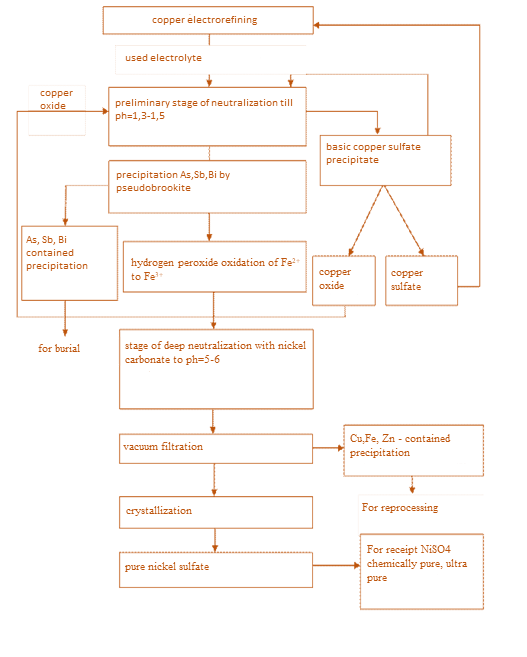
\includegraphics[width=0.8\textwidth]{media/chem2/image17}
	\caption*{}
\end{figure}


{\bfseries Fig. 1 -Technological scheme of the integrated processing of
copper electrolyte to obtain nickel sulfate}

{\bfseries Materials and methods.} The object of large-scale laboratory
tests is the technological copper-containing sulfuric solution of the
corporation "KAZAKHMYS SMELTING" (Republic of Kazakhstan, city of
Balkhash). The quantitative content of the main components of the
process solution (Cu, Ni, H\textsubscript{2}SO\textsubscript{4}, As, Sb,
Bi, Fe, Zn) was determined on a SPEKS SSP-705-4 scanning
spectrophotometer, as well as on a laser atomic emission spectrometer
SPEKS LAES MATRIX CONTINUUM (Closed Joint Stock «Company Spectroscopic
Systems» Russian Federation, 2016) , the results of which are presented
in Table 1.

Large-scale laboratory tests were carried out with a volume of the
working solution equal to 500 ml.

{\bfseries Table 1 - Electrolytecomposition}

% \begin{longtable}[]{@{}
%   >{\raggedright\arraybackslash}p{(\columnwidth - 16\tabcolsep) * \real{0.1990}}
%   >{\raggedright\arraybackslash}p{(\columnwidth - 16\tabcolsep) * \real{0.1225}}
%   >{\raggedright\arraybackslash}p{(\columnwidth - 16\tabcolsep) * \real{0.1072}}
%   >{\raggedright\arraybackslash}p{(\columnwidth - 16\tabcolsep) * \real{0.1073}}
%   >{\raggedright\arraybackslash}p{(\columnwidth - 16\tabcolsep) * \real{0.0918}}
%   >{\raggedright\arraybackslash}p{(\columnwidth - 16\tabcolsep) * \real{0.0918}}
%   >{\raggedright\arraybackslash}p{(\columnwidth - 16\tabcolsep) * \real{0.0921}}
%   >{\raggedright\arraybackslash}p{(\columnwidth - 16\tabcolsep) * \real{0.0917}}
%   >{\raggedright\arraybackslash}p{(\columnwidth - 16\tabcolsep) * \real{0.0965}}@{}}
% \toprule\noalign{}
% \endhead
% \bottomrule\noalign{}
% \endlastfoot
% Component & Cu & Ni & H\textsubscript{2}SO\textsubscript{4} & As & Sb &
% Bi & Fe & Zn \\
% g/l & 51.20 & 16.98 & 95.88 & 14.04 & 8.63 & 5.78 & 9.42 & 9.17 \\
% \end{longtable}

{\bfseries Results and discussion.} Based on known methods for processing
copper electrolyte {[}12,14{]}, 500 ml of water was added to a copper
electrolyte with a volume of 500 ml, and treated with 96 g of copper
(II) oxide in a molar ratio CuO:Cu = 3:1. The reaction mass was heated
in a thermostated cell to 98\textsuperscript{0}С with constant stirring
for four hours. The solution volume was decreased by 2 times at the end
of the neutralizing process. The solution was filtered in a hot state,
resulting in a precipitate of basic dark green copper sulfate weighing
406.59 g on the filter. Further, basic copper sulfate obtained in an
amount of 348.3 g was used for subsequent neutralization of copper
electrolyte with a volume of 500 ml for each experiment.

The neutralization of free sulfuric acid was carried out for 15 min in a
thermostated cell at a temperature of 85\textsuperscript{0}С. The
solution pH was monitored during the experiment until its values reached
1.31. Hot solutions were subjected to vacuum filtration, and then cooled
to a temperature of 20\textsuperscript{0}С. Copper sulfate weighing ≈
43.8 g was obtained in each experiment. The solutions were analyzed for
the residual content of sulfuric acid, copper, nickel, and arsenic. The
average values of the investigation results are shown in Table 2.

{\bfseries Table 2 - Results of the copper electrolyte neutralization
process}

{\bfseries (Cu\textsubscript{3}(OH)\textsubscript{4}SO\textsubscript{4}:H\textsubscript{2}SO\textsubscript{4})
= 2:1; t = 85\textsuperscript{0}С; τ = 15 min)}

% \begin{longtable}[]{@{}
%   >{\raggedright\arraybackslash}p{(\columnwidth - 10\tabcolsep) * \real{0.1384}}
%   >{\raggedright\arraybackslash}p{(\columnwidth - 10\tabcolsep) * \real{0.1562}}
%   >{\raggedright\arraybackslash}p{(\columnwidth - 10\tabcolsep) * \real{0.1803}}
%   >{\raggedright\arraybackslash}p{(\columnwidth - 10\tabcolsep) * \real{0.1801}}
%   >{\raggedright\arraybackslash}p{(\columnwidth - 10\tabcolsep) * \real{0.1800}}
%   >{\raggedright\arraybackslash}p{(\columnwidth - 10\tabcolsep) * \real{0.1649}}@{}}
% \toprule\noalign{}
% \multicolumn{2}{@{}>{\raggedright\arraybackslash}p{(\columnwidth - 10\tabcolsep) * \real{0.2946} + 2\tabcolsep}}{%
% \begin{minipage}[b]{\linewidth}\raggedright
% рН of working solution
% \end{minipage}} &
% \multirow{2}{=}{\begin{minipage}[b]{\linewidth}\raggedright
% H\textsubscript{2}SO\textsubscript{4}(g/l)
% \end{minipage}} &
% \multirow{2}{=}{\begin{minipage}[b]{\linewidth}\raggedright
% Cu(g/l)
% \end{minipage}} &
% \multirow{2}{=}{\begin{minipage}[b]{\linewidth}\raggedright
% Ni(g/l)
% \end{minipage}} &
% \multirow{2}{=}{\begin{minipage}[b]{\linewidth}\raggedright
% As(g/l)
% \end{minipage}} \\
% \begin{minipage}[b]{\linewidth}\raggedright
% Before experiment
% \end{minipage} & \begin{minipage}[b]{\linewidth}\raggedright
% After experiment
% \end{minipage} \\
% \midrule\noalign{}
% \endhead
% \bottomrule\noalign{}
% \endlastfoot
% 0.08 & 1.31 & 2.79 & 31.0 & 16.70 & 14.03 \\
% \end{longtable}

The obtained copper-nickel mother liquors were re-diluted with water 2
times and subjected to de-curing with copper (II) oxide. Width of the
confidence interval according to the Cochran criterion for copper
content ∆= 0.18δ = 2∆.

The resulting basic copper sulfate weighing 24.99 g was used to
neutralize the next portion of the electrolyte. The main copper sulfate
is also a raw material for the production of copper oxide, copper
sulfate. The resulting solutions, after neutralization and de-curing of
the electrolyte, were analyzed for the residual content of sulfuric
acid, copper, nickel, and arsenic. The average values of the analysis
results are shown in Table 3.

{\bfseries Table 3 -} {\bfseries Copper electrolyte dressing from copper
results\\
(CuO:Cu= 3:1; t = 98\textsuperscript{0}С; τ = 4 hour)}

% \begin{longtable}[]{@{}
%   >{\raggedright\arraybackslash}p{(\columnwidth - 14\tabcolsep) * \real{0.1375}}
%   >{\raggedright\arraybackslash}p{(\columnwidth - 14\tabcolsep) * \real{0.1375}}
%   >{\raggedright\arraybackslash}p{(\columnwidth - 14\tabcolsep) * \real{0.1524}}
%   >{\raggedright\arraybackslash}p{(\columnwidth - 14\tabcolsep) * \real{0.1650}}
%   >{\raggedright\arraybackslash}p{(\columnwidth - 14\tabcolsep) * \real{0.0007}}
%   >{\raggedright\arraybackslash}p{(\columnwidth - 14\tabcolsep) * \real{0.1738}}
%   >{\raggedright\arraybackslash}p{(\columnwidth - 14\tabcolsep) * \real{0.1175}}
%   >{\raggedright\arraybackslash}p{(\columnwidth - 14\tabcolsep) * \real{0.1156}}@{}}
% \toprule\noalign{}
% \multicolumn{2}{@{}>{\raggedright\arraybackslash}p{(\columnwidth - 14\tabcolsep) * \real{0.2750} + 2\tabcolsep}}{%
% \begin{minipage}[b]{\linewidth}\raggedright
% рН of working solution
% \end{minipage}} &
% \multirow{2}{=}{\begin{minipage}[b]{\linewidth}\raggedright
% H\textsubscript{2}SO\textsubscript{4}(g/l)
% \end{minipage}} &
% \multicolumn{3}{>{\raggedright\arraybackslash}p{(\columnwidth - 14\tabcolsep) * \real{0.3395} + 4\tabcolsep}}{%
% \begin{minipage}[b]{\linewidth}\raggedright
% Cu(g/l)
% \end{minipage}} &
% \multirow{2}{=}{\begin{minipage}[b]{\linewidth}\raggedright
% Ni(g/l)
% \end{minipage}} &
% \multirow{2}{=}{\begin{minipage}[b]{\linewidth}\raggedright
% As(g/l)
% \end{minipage}} \\
% \begin{minipage}[b]{\linewidth}\raggedright
% Before experiment
% \end{minipage} & \begin{minipage}[b]{\linewidth}\raggedright
% After experiment
% \end{minipage} & &
% \multicolumn{2}{>{\raggedright\arraybackslash}p{(\columnwidth - 14\tabcolsep) * \real{0.1657} + 2\tabcolsep}}{%
% \begin{minipage}[b]{\linewidth}\raggedright
% Before experiment
% \end{minipage}} & \begin{minipage}[b]{\linewidth}\raggedright
% After
% 
% experiment
% \end{minipage} \\
% \midrule\noalign{}
% \endhead
% \bottomrule\noalign{}
% \endlastfoot
% 1.31 & 2.37 & 0.21 & 31.0 &
% \multicolumn{2}{>{\raggedright\arraybackslash}p{(\columnwidth - 14\tabcolsep) * \real{0.1745} + 2\tabcolsep}}{%
% 0.79} & 16.5 & 14.01 \\
% \end{longtable}

Copper-bearing sediments were identified by IR spectroscopic analysis
(Figure 2). According to reference data {[}15{]}, intense absorption
bands at 1106-1366 cm\textsuperscript{-1} and 451-621
cm\textsuperscript{-1} are related to the sulfate ion. Also, a band in
the region of 3140 - 3433 cm\textsuperscript{-1} is characteristic of
stretching vibrations of OH-groups, and absorption bands at 1340-1627
cm\textsuperscript{-1} associated with the presence of water molecules
in a highly hydrated sediment. Based on the data of the IR spectra of
the precipitate and the results of photometric analysis for copper, it
was established that the resulting precipitate is the main copper
sulfate Cu\textsubscript{3}(OH)\textsubscript{4}SO\textsubscript{4}.

\begin{figure}[H]
	\centering
	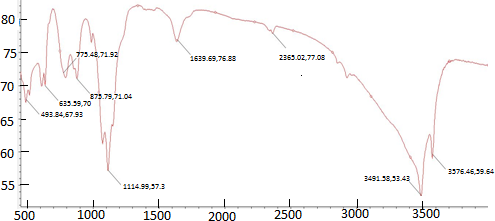
\includegraphics[width=0.8\textwidth]{media/chem2/image18}
	\caption*{}
\end{figure}


{\bfseries Fig. 2 - IR spectrogram of a copper-bearing precipitate}

Additionally, the analysis for the content of impurities in the
resulting sediment was carried out on a laser atomic emission
spectrometer SPEX LAES MATRIX CONTINUUM (Figure 3). As can be seen from
the spectrogram, intense green peaks are observed, which correspond to
copper ions. The presence of such impurities as iron, zinc, arsenic,
antimony, bismuth in the composition of the precipitate is not observed
on the spectrogram. Thus, the resulting basic copper sulfate does not
contain foreign impurities of other metals and is a chemically pure
compound.

\begin{figure}[H]
	\centering
	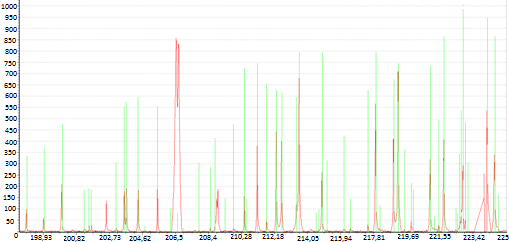
\includegraphics[width=0.8\textwidth]{media/chem2/image19}
	\caption*{}
\end{figure}


{\bfseries Fig. 3 ‒ Laser spectrogram of copper-bearing sediment}

The deposition of arsenic, antimony and bismuth with pseudobrookite was
carried out in a thermostated cell at a temperature of
60\textsuperscript{0}С, with a given concentration of sulfuric acid with
constant stirring for one hour. We used the resulting solutions with a
volume of 182 ml each. A weighed portion of pseudobrookite was taken
equal to the ratio of the precipitant to arsenic 1:1 in the amount of
14.01 g and fed in two portions (DRP= 2). Then the solution was filtered
while hot, the resulting filtrates with a volume of 165 ml were analyzed
for the residual arsenic content, antimony and bismuth in them. The
results of analyzes for the residual content of antimony, bismuth
arsenic, shown in Table 4, showed that their content in solutions is
reduced to trace amounts, i.e., the resulting solutions are almost
completely purified from them.

For the oxidation of Fe\textsuperscript{2+} ions to
Fe\textsuperscript{3+}, 3.1 ml of hydrogen peroxide was introduced into
solutions with a volume of 158 ml of each experiment. Then the solutions
were stirred for one hour in a thermostated cell at a temperature of
50-55\textsuperscript{0}С. At the end of the experiments, the solutions
were cooled and analyzes were carried out for the total iron content and
for Fe\textsuperscript{3+}, the results of all analyzes of the
experiments were averaged (g/l): C(Fe\textsubscript{tot}) = 6,035;
C(Fe\textsuperscript{3+}) = 6,030. Under these conditions, complete
oxidation of Fe\textsuperscript{2+}toFe\textsuperscript{3+}ions is
achieved.

In order to purify working solutions from ions of copper, iron, zinc
(C(Zn\textsuperscript{2+}) = 6.7 g/l; C(Fe\textsuperscript{3+}) = 6.03
g/l; C(Cu\textsuperscript{2+}) = 0.79 g/l) a solution of phosphoric acid
in the amount of 13.8 mlwere added in them.

Then the solutions were heated with stirring to 85\textsuperscript{0}С,
added H\textsubscript{2}O in an amount of 25.5 ml, and the solutions
were heated to 90\textsuperscript{0}С. Nickel carbonate weighing 12.62 g
was added to the heated solution in portions. The solutions were
constantly stirred and kept at a temperature of 90\textsuperscript{0}С
for 1.5 hours. With the addition of each portion of nickel carbonate, a
sample was taken and the pH of the solutions was measured. Nickel
carbonate was added until a pH of about 5.98 was reached.

Insoluble precipitates and unreacted nickel carbonate were separated by
vacuum filtration. 0.1 ml of concentrated sulfuric acid was added to the
filtrate, after the addition of which the pH of the solutions reached a
value of ≈ 2.39.

At the end of the process, the solution was subjected to vacuum
filtration while hot. Insoluble sediments weighing 2.19 g remained on
the filter. Then the test solution was cooled to a temperature of
20-23\textsuperscript{0}С. Crystals of nickel sulfate began to grow in
the solution on the seventh day. The crystals were separated from the
working solution by filtration, washed with distilled water, dried, and
weighed. As a result, we got 66.35 g heptahydrate nickel sulfate, on
average in each experiment.

{\bfseries Table 4 ‒ The results of the precipitation of arsenic, antimony
and bismuth by}

{\bfseries pseudobrookite(\emph{t =} 60 \textsuperscript{0}C; \emph{τ =} 1
hour; DRP= 2)}

% \begin{longtable}[]{@{}
%   >{\raggedright\arraybackslash}p{(\columnwidth - 14\tabcolsep) * \real{0.0893}}
%   >{\raggedright\arraybackslash}p{(\columnwidth - 14\tabcolsep) * \real{0.1650}}
%   >{\raggedright\arraybackslash}p{(\columnwidth - 14\tabcolsep) * \real{0.1242}}
%   >{\raggedright\arraybackslash}p{(\columnwidth - 14\tabcolsep) * \real{0.1245}}
%   >{\raggedright\arraybackslash}p{(\columnwidth - 14\tabcolsep) * \real{0.1243}}
%   >{\raggedright\arraybackslash}p{(\columnwidth - 14\tabcolsep) * \real{0.1243}}
%   >{\raggedright\arraybackslash}p{(\columnwidth - 14\tabcolsep) * \real{0.1244}}
%   >{\raggedright\arraybackslash}p{(\columnwidth - 14\tabcolsep) * \real{0.1242}}@{}}
% \toprule\noalign{}
% \multirow{2}{=}{\begin{minipage}[b]{\linewidth}\raggedright
% №
% 
% Experiment
% \end{minipage}} &
% \multirow{2}{=}{\begin{minipage}[b]{\linewidth}\raggedright
% Fe\textsubscript{2}TiO\textsubscript{5}:As
% \end{minipage}} &
% \multicolumn{3}{>{\raggedright\arraybackslash}p{(\columnwidth - 14\tabcolsep) * \real{0.3729} + 4\tabcolsep}}{%
% \begin{minipage}[b]{\linewidth}\raggedright
% Concentration after experiment, (g/l)
% \end{minipage}} &
% \multicolumn{3}{>{\raggedright\arraybackslash}p{(\columnwidth - 14\tabcolsep) * \real{0.3728} + 4\tabcolsep}@{}}{%
% \begin{minipage}[b]{\linewidth}\raggedright
% Degree of precipitation, \%
% \end{minipage}} \\
% & & \begin{minipage}[b]{\linewidth}\raggedright
% As
% \end{minipage} & \begin{minipage}[b]{\linewidth}\raggedright
% Sb
% \end{minipage} & \begin{minipage}[b]{\linewidth}\raggedright
% Bi
% \end{minipage} & \begin{minipage}[b]{\linewidth}\raggedright
% As
% \end{minipage} & \begin{minipage}[b]{\linewidth}\raggedright
% Sb
% \end{minipage} & \begin{minipage}[b]{\linewidth}\raggedright
% Bi
% \end{minipage} \\
% \midrule\noalign{}
% \endhead
% \bottomrule\noalign{}
% \endlastfoot
% 1 & 0.5:1 & 0.070 & 0.0023 & 0.0011 & 99.15 & 99.85 & 99.88 \\
% 2 & 0.8:1 & 0.032 & 0.0016 & 0.0005 & 99.67 & 99.89 & 99.90 \\
% 3 & 1:1 & Traces & Traces & Traces & 99.99 & 99.99 & 99.99 \\
% 4 & 1.2:1 & Traces & Traces & Traces & 99.99 & 99.99 & 99.99 \\
% 5 & 1.5:1 & Traces & Traces & Traces & 99.99 & 99.99 & 99.99 \\
% \end{longtable}

Calculated the average yield of the target product of nickel sulfate.
The theoretical mass of the target product according to calculations
from the reaction equations:

NiCO\textsubscript{3}→ NiO +CO\textsubscript{2}↑ (4)

NiO + H\textsubscript{2}SO\textsubscript{4} → NiSO\textsubscript{4} +
H\textsubscript{2}O (5)

NiSO\textsubscript{4} + 7H\textsubscript{2}O → NiSO\textsubscript{4} ∙
7H\textsubscript{2}O (6)

was 92.59 g. The average yield of the target product of nickel sulfate
was 71.66\% of the theoretically possible.

Analysis of the obtained IR spectra of nickel sulfate crystals (Figure
4) confirmed the absence of copper, iron and zinc impurities in nickel
sulfate crystals. In the figure, one can see intense bands at 1106-1366
cm\textsuperscript{-1} and 451-621 cm\textsuperscript{-1}, which
corresponds to the absorption bands of sulfate ions; in addition, bands
are observed in the region of 1340-1670 cm\textsuperscript{-1},
characteristic of the presence of crystallized water in a highly
hydrated sediment. It is also possible to observe low-intensity
absorption bands in the region of 3440-3470 cm\textsuperscript{-1}
characteristic of stretching vibrations of OH-groups, and an
insignificant absorption band at 2830-2850 cm\textsuperscript{-1}related
to the carbonate ion {[}15{]}. That is, the obtained crystals were
confirmed to be nickel sulfate
(NiSO\textsubscript{4}∙7H\textsubscript{2}O).

\begin{figure}[H]
	\centering
	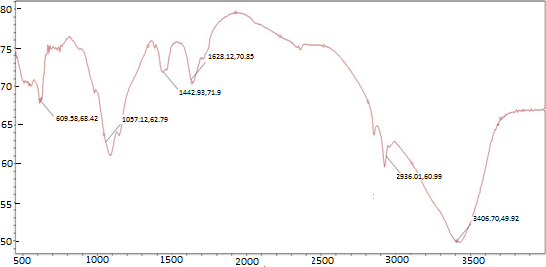
\includegraphics[width=0.8\textwidth]{media/chem2/image20}
	\caption*{}
\end{figure}


{\bfseries Fig. 4 - IR spectra of crystals of the obtained nickel sulfate}

The nickel sulfate obtained as a result of large-scale laboratory tests,
as noted earlier, does not contain metal impurities, and can be used as
a raw material for obtaining nickel sulfate of reagent grade, special
grade, which in turn confirms the technological significance of the
tests carried out and the effectiveness of the technological scheme of
the new technology for processing copper electrolyte (Figure 1).

{\bfseries Conclusion.} The large-scale laboratory tests have shown the
efficiency of the new technology of processing copper electrolyte and
the possibility, along with obtaining marketable copper products: basic
copper sulfate, copper oxide, copper sulfate, to expand the range of
products of vitriol processing based on nickel - nickel sulfate. The
results of large-scale laboratory tests can serve as initial data for
planning and conducting subsequent production tests of a new technology
of processing copper electrolyte.

{\bfseries References}

\begin{enumerate}
\def\labelenumi{\arabic{enumi}.}
\item
  Wang, Biao Liu , Xue-wen Wang , Yu-qi Meng , Xing-ming Wang , Ming-yu
  Wang Separation and recovery of Ni from copper electrolyte by
  crystallization of nickel ammonium sulfate double salt //Transactions
  of nonferrous metals. -Sociaty of China, 2022.- Vol. 32(11).- P.
  3780-3789. DOI
  \href{http://dx.doi.org/10.1016/S1003-6326(22)66057-6}{10.1016/S1003-6326(22)66057-6}.
\item
  Kholikulov D.B., Abdurahmonov S., Boltaev O.N., Matkarimov
  S.T{\bfseries .} Separation of metals from technological solutions.
  Copper production // International Journal of Emerging Trends in
  Engineering Research\emph{.-} 2020. - Vol. 8(7). - P. 3557-3561. DOI
  10.30534/ijeter/2020/110872020
\end{enumerate}

3.Sokolov A.Ju., Shhelokova E. A., Voroncov K. A., Kasikov A. G.
Kompleksnaja pererabotka otrabotannogo mednogo jelektrolita//Trudy
Kol' skogo nauchnogo centra RAN.-2023.- T. 14(1) - S.
229-233. DOI 10.37614/2949-1215.2023.14.1.041. {[}in Russian{]}

4.Narembekova A., Tokenova Z.Sh. Al' ternativnaja
tehnologija pererabotki med' soderzhashhih
rastvorov//Trudy universiteta.- 2020. -№3 (80).- S.34-38. DOI
10.52209/1609-1825\_2020\_3\_33.

{[}in Russian{]}

5.Kholikulov D., Boltaev O. Separation of Copper from Technological
Solutions to the Production of Copper Sulphate // International Journal
of Advanced Research in Science, Engineering and Technology. -2020.
-Vol. 7(1). -P. 12626-12631.

6.Deng Z., Oraby E., Li H., Eksteen J. Extraction of Copper from
Chalcopyrite Using Alkaline Glycine--Ammonia
Solutions//Minerals.-2022.-Vol. 12(12): 1507. DOI 10.3390/min12121507.

7.Moazzami Y., Shafaei Tonkaboni S.Z., Gharabaghi M. Leaching Kinetics
of Chalcopyrite Concentrate by Ionic Liquids // Iranian Journal of
Materials Science and Engineering. -2022. -Vol. 19(4). DOI
10.22068/ijmse.2812

8.Sergeev S. Mednye problemy cvetnoj metallurgii // Sbornik nauchnyh
trudov Kazahstana. -- Almaty, 2010.-№ 3.- S. 1-3. {[}in Russian{]}

9. Harchenko E.M., Zhumashev K.Zh. Izuchenie nauchno-tehnologicheskih
osnov sovmestnoj pererabotki otval' nyh mednyh shlakov i
obrabotannogo mednogo jelektrolita // Vestnik JuUrGU. Serija
«Metallurgija». -2011. -№ 36.- № 17.- S.18-22. {[}in Russian{]}

10. Sadykov R. R., Shulga E. V., Petrov A. F., Kotukhov S. B. Two-stage
neutralization method to process copper-nickel sulfurous solutions of
the Copper Plant, Polar Division of PC MMC Norilsk Nickel //Tsvetnye
Metally.-2015.- Vol.6. -P. 54 - 59. DOI 10.17580/tsm.2015.06.11.

11. Liu X., He Y., Zhao Z., Chen X. Study on removal of copper from
nickel-copper mixed solution by membrane
electrolysis//Hydrometallurgy.-2018.-Vol.180.- P.153-157.

DOI 10.1016/j.hydromet.2018.07.019.

12.Omarov H.B., Әbsәt Z.B., Aldabergenova S.K., Muzapparov A.A., Umanova
I.K. Sposob pererabotki mednogo jelektrolita: pat. 3082 Respublika
Kazahstan. - № 2018/0029.2; zajavl. 15.01.2018; opubl. 10.09.2018, Bjul.
№ 34. {[}in Russian{]}

13.Bakeev M.I., Narembekova A., Zharmenov A.A., Zhumashev K.Zh.,
Turumbetov U.A. Sposob pererabotki mednogo jelektrolita: pat. 15985
Respublika Kazahstan. - № 2003/0815.1; zajavl. 16.06.2003; opubl.
15.07.2005, Bjul. № 7. {[}in Russian{]}

14.Omarov H.B., Absat Z.B., Aldabergenova S.K., Rahimzhanova N.Zh.,
Muzapparov A.A. Issledovanie processa osazhdenija
mysh' jaka iz mednogo jelektrolita psevdobrukitom //
Izvestija vuzov.Cvetnaja metallurgija.-2017.-№ 6. -S.11-19. DOI
10.17073/0021-3438-2017-6-11-19. {[}in Russian{]}

15.Spectral Database for Organic Compounds SDBS. URL:
\url{http://sdbs.db.aist.go.jp/sdbs/cgi-bin/direct_frame_top.cgi} .Date
of address: 27.12.2024

\emph{{\bfseries Information about the authors}}

Omarov K.B. - Doctor of Technical Sciences, Professor, Kazakh University
of Technology and Business named after K.Kulazhanov, Astana, Kazakhstan,
e-mail:
\href{mailto:homarov1963@mail.ru}{\nolinkurl{homarov1963@mail.ru}};

Nurgaliyev N.U. - Candidate of Chemical Sciences, Associate Professor,
Kazakh University of Technology and Business named after K.Kulazhanov,
Astana„ Kazakhstan, e-mail:nurgaliev\_nao@mail.ru;

Mostovoy A.S. - Candidate of technical sciences, Associate professor,
Saratov State Technical University named after Y. Gagarin, Saratov,
Russia, e-mail: mostovoy19@rambler.ru;

Absat Z. B. {\bfseries -} Candidate of Chemical Sciences, Associate
Professor of the Department of Chemical Technology and Petrochemistry of
the Karaganda University named after Academician E.A. Buketov,
Karaganda, Kazakhstan, e-mail: zaure.absat.76@mail.ru;

Алдабергенова С.К. - Candidate of Chemical Sciences, Associate
Professor, Karaganda University named after Academician E.A. Buketov,
Karaganda, Kazakhstan, e-mail: aldsau@mail.ru;

Nurtai Zh.T. - PhD, Associate Professor, Kazakh University of Technology
and Business named after K.Kulazhanov, Astana, Kazakhstan, e-mail:
zhadira\_nurtai@mail.ru;

Zhunussova E.B. - Candidate of Technical Sciences, Associate Professor,
Kazakh University of Technology and Business named after K.Kulazhanov,
Astana, Kazakhstan, е-mail: tahmina.66@mail.ru;

Zhumabekova A.K. - Candidate of Chemical sciences, Associate Professor,
Kazakh University of Technology and Business named after K.Kulazhanov,
Astana, Kazakhstan, e-mail: zhumabekova\_ak@mail.ru;

Issabayeva М.А. - Candidate of Chemical Sciences, Professor, Toraigyrov
University, Pavlodar, Kazakhstan, e-mail: isabaeva.manar@mail.ru

\emph{{\bfseries Сведения об авторах}}

Омаров Х.Б. - доктор технических наук, профессор, Казахский университет
технологии и бизнеса им. К.Кулажанова, Астана, Казахстан, e-mail:
homarov1963@mail.ru;

Нургалиев Н.У. - кандидат химических наук, ассоциированный профессор,
Казахский университет технологии и бизнеса имени К.Кулажанова, Астана,
Казахстан, e-mail: nurgaliev\_nao@mail.ru;

Мостовой А.С. - кандидат технических наук, ассоциированный профессор,
Саратовский государственный технический университет имени Ю.А. Гагарина,
Саратов, Россия, e-mail: mostovoy19@rambler.ru;

Абсат З.Б. - кандидат химических наук, ассоциированный профессор,
Карагандинский университет им. академика Е.А.Букетова, Караганда,
Казахстан, e-mail: zaure.absat.76@mail.ru;

Алдабергенова С.К. - кандидат химических наук, ассоциированный
профессор,Карагандинский университет им. академика Е.А.Букетова,
Караганда, Казахстан, e-mail:
\href{mailto:aldsau@mail.ru}{\nolinkurl{aldsau@mail.ru}}

Нұртай Ж.Т. - доктор PhD, ассоциированный профессор, Казахский
университет технологии и бизнеса имени К.Кулажанова, Астана, Казахстан,
e-mail: zhadira\_nurtai@mail.ru;

Жунусова Э.Б. - кандидат технических наук, ассоциированный профессор,
Казахский университет технологии и бизнеса им. К.Кулажанова, Астана,
Казахстан, e-mail: tahmina.66@mail.ru;

Жумабекова А.К. - кандидат химических наук, ассоциированный профессор,
Казахский университет технологии и бизнеса им. К.Кулажанова, Астана,
Казахстан, e-mail:
\href{mailto:zhumabekova_ak@mail.ru}{\nolinkurl{zhumabekova\_ak@mail.ru}};

Исабаева М.А. - кандидат химических наук, профессор, Торайгыров
университет, Павлодар, Казахстан, e-mail: isabaeva.manar@mail.ru